% METODOLOGIA------------------------------------------------------------------

\chapter{Metodologia}
\label{chap:metodologia}

A metodologia empregada neste trabalho está organizada nos seguintes passos principais:

\begin{description}
\item[Etapa 1] Aquisição da base de dados BOSSBase~\cite{bas2011break}.
\item[Etapa 2] Aplicação dos algoritmos HUGO, MiPOD e S-UNIWARD nas imagens da base BOSSBase para criar as estego imagens, as quais irão compor as bases de treinamento e teste.
\item[Etapa 3] Realização do procedimento de esteganálise utilizando a abordagem tradicional: extração de descritores (SRM) e classificação (\textit{Ensemble of Classifiers}).
\item[Etapa 4] Realização do procedimento de esteganálise utilizando-se uma CNN.
\item[Etapa 5] Análise comparativa dos resultados obtidos a partir das Etapas 3 e 4. Os resultados desta etapa serão discutidos em detalhes no próximo capítulo.
\end{description}

As seções a seguir detalham como esses passos serão realizados.

\section{Base de Dados}
\label{sec:database}

Neste trabalho foi utilizada a base de imagens denominada BOSSBase (v1.01)\footnote{Disponível em: \url{http://dde.binghamton.edu/download/ImageDB/BOSSbase_1.01.zip} (acessado em 11/2017).}, a qual  foi criada para a competição de esteganálise \textit{Break Our Steganographic System} (BOSS) \cite{bas2011break}. É composta por 10000 imagens sem compressão, em escala de cinza, com dimensões 512x512 e provenientes de 7 câmeras diferentes, produzindo assim, padrões de ruídos de captação diferentes para não gerar especializações em algoritmos de esteganografia que utilizam abordagens adaptativas e exploram esses ruídos.

A competição BOSS buscava inicialmente incentivar a criação de algoritmos de esteganálise para quebrar o HUGO. A sua importância na área de esteganografia se consolidou após o grupo vencedor, denominado \textit{"HUGO breakers"}, propor o uso dos descritores SRM.

Alguns exemplos da base de dados BOSS podem ser vistos na Figura~\ref{fig:bossexample}.

\begin{figure}[h]
	\center
	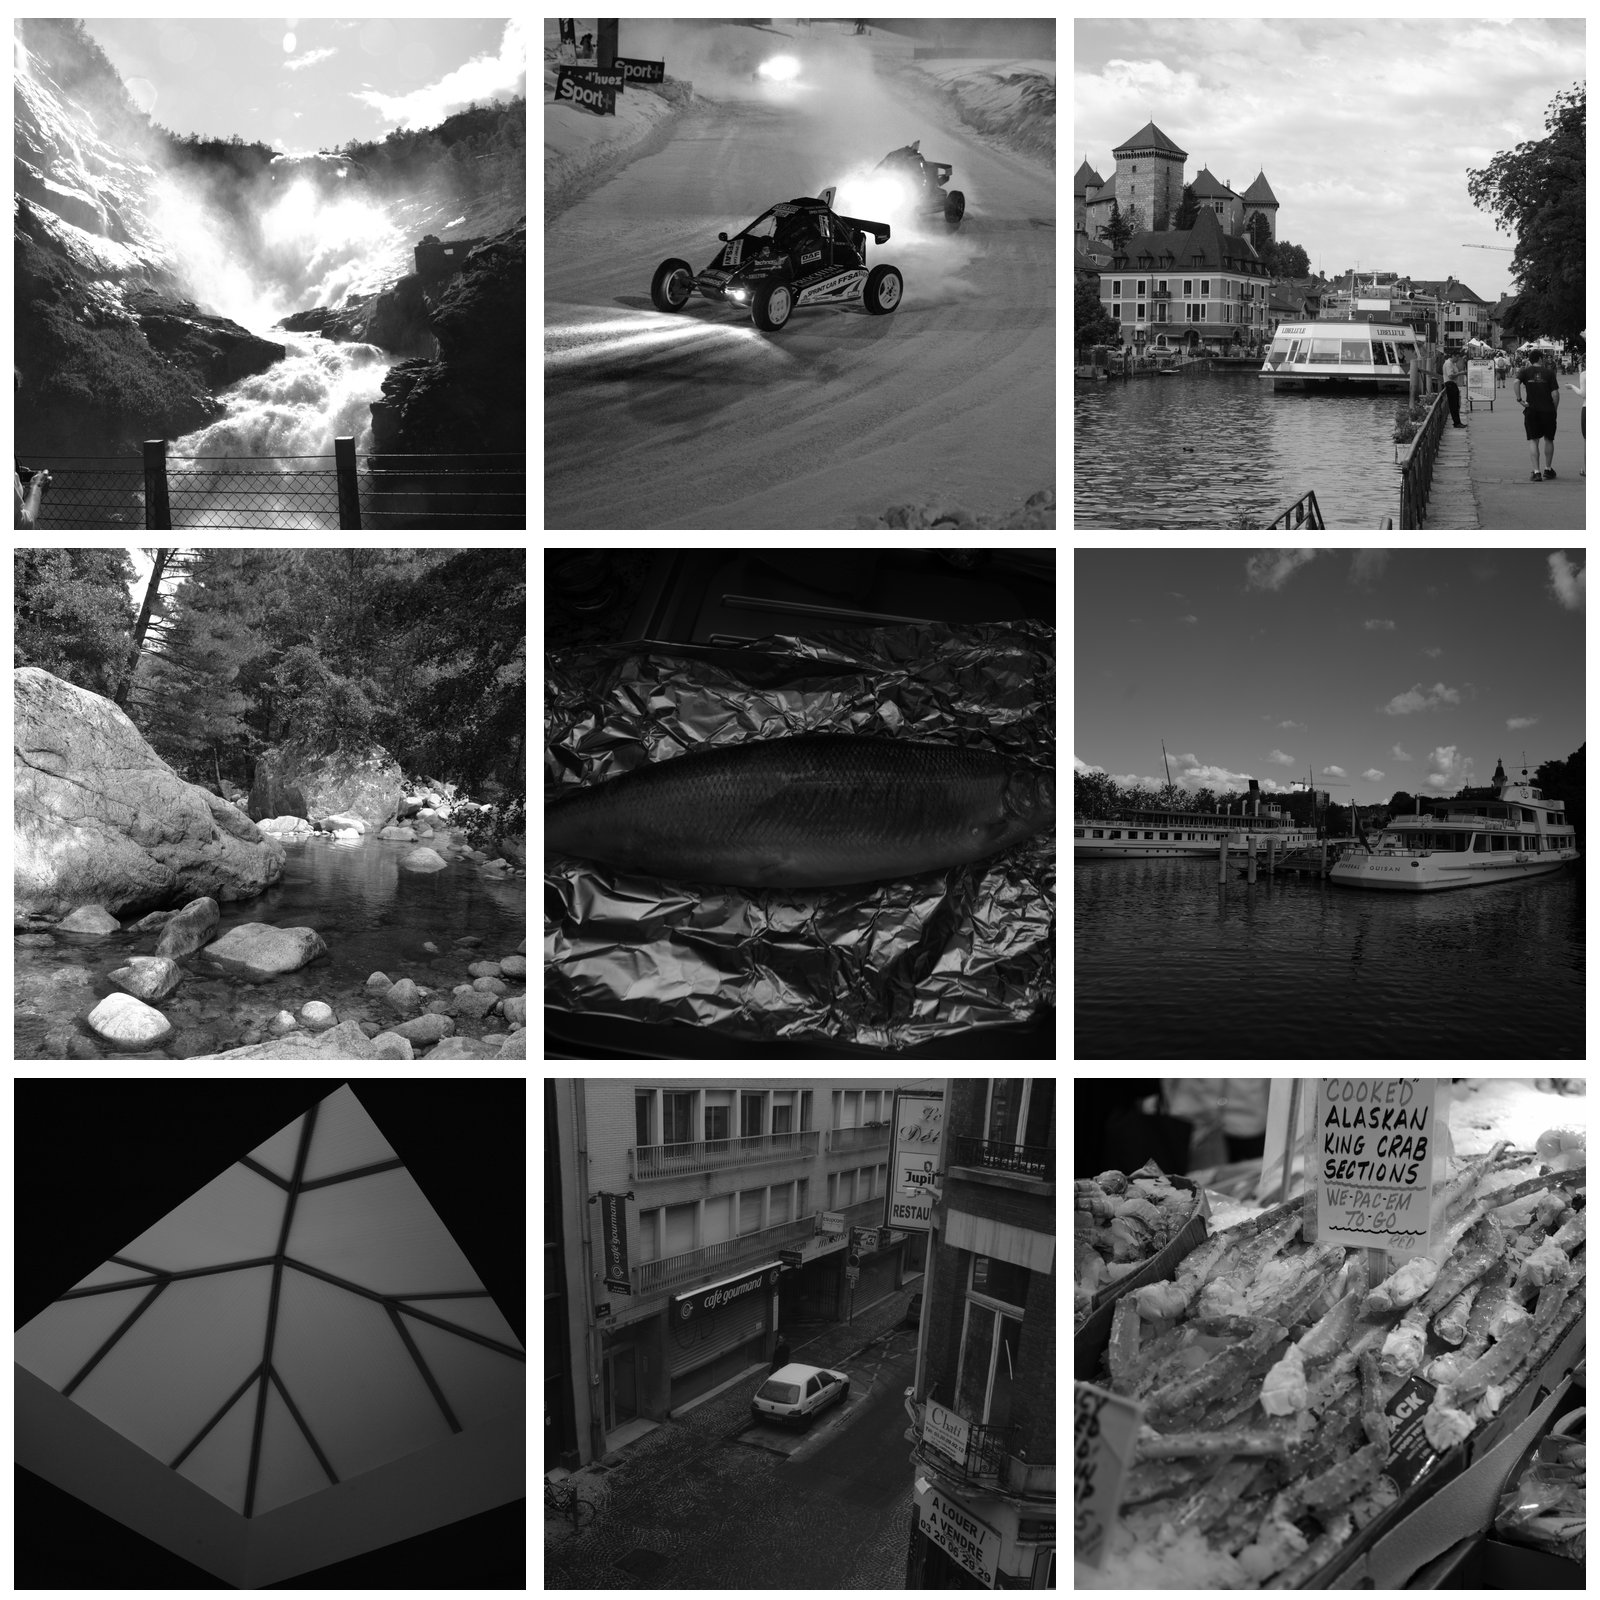
\includegraphics[width=0.8\textwidth]{dados/figuras/exemplo-boss.png}
	\caption{Exemplos de amostras da base BOSS.}
	\label{fig:bossexample}
\end{figure}

\section{Criação das Estego Imagens}
\label{sec:impl-alg}

Visando criar diferentes cenários de treinamento e teste, os algoritmos de esteganografia HUGO~\cite{hugo}, S-UNIWARD~\cite{holub2014universal} e MiPOD~\cite{sedighi2016content} (Subseções~\ref{subsec:hugo}~-~\ref{subsec:mipod}) foram aplicados nas imagens da base de dados BOSSBase, considerando-se diferentes parâmetros. Tais cenários permitem avaliar o desempenho das abordagens de esteganálise consideradas neste trabalho, tanto ao comparar a combinação de diferentes algoritmos de esteganografia nas etapas de treinamento e teste quando ao avaliar o impacto da utilização de diferentes \textit{payloads}.

Os cenários de treinamento são listados na Tabela~\ref{tab:cenariosTrain}. Em resumo, as 5000 imagens iniciais da BOSSBase foram utilizadas para aplicação dos algoritmos HUGO, S-UNIWARD e MiPOD para quatro diferentes \textit{payloads}: 0.1, 0.2, 0.4 e 0.6. Portanto, foram criados 12 diferentes conjuntos de treinamento, os quais serão referenciados no decorrer deste trabalho pela sigla presente na primeira coluna (formada pela primeira letra do nome do algoritmo seguida por um valor que representa o \textit{payload}).

\begin{table}[!htb]
\centering
\caption{Cenários de treinamento.}
\label{tab:cenariosTrain}
\begin{tabular}{|c|c|c|}
\hline
Nomenclatura& Algoritmo & \textit{Payload}\\ \hline
H1 & \multirow{4}{*}{HUGO} & 0.1 \\ \cline{1-1} \cline{3-3} 
H2 &                   &  0.2\\ \cline{1-1} \cline{3-3} 
H4 &                   &  0.4\\ \cline{1-1} \cline{3-3} 
H6 &                   &  0.6\\ \hline
S1 & \multirow{4}{*}{S-UNIWARD} & 0.1 \\ \cline{1-1} \cline{3-3} 
S2 &                   &  0.2\\ \cline{1-1} \cline{3-3} 
S4 &                   &  0.4\\ \cline{1-1} \cline{3-3} 
S6 &                   &  0.6\\ \hline
M1 & \multirow{4}{*}{MiPOD} & 0.1 \\ \cline{1-1} \cline{3-3} 
M2 &                   & 0.2 \\ \cline{1-1} \cline{3-3} 
M4 &                   &  0.4\\ \cline{1-1} \cline{3-3} 
M6 &                   &  0.6\\ \hline
\end{tabular}
\end{table}
% \vskip -0.5cm
As estego imagens para os testes foram geradas a partir das 5000 últimas imagens da BOSSBase, criando os cenários de teste listados na Tabela~\ref{tab:cenariosTest}. Observe que, além da variação do \textit{payload}, foram utilizados também diferentes valores de STC. % para os algoritmos HUGO e S-UNIWARD. 
Os parâmetros para o HUGO (STC, $\gamma$ e $\sigma$) foram extraídos de \citeonline{hugo}\footnote{Foi gerado também um cenário do HUGO com STC de altura 10, $\gamma = 1$ e $\sigma = 5$. Porém, como não houve uma variação significativa nos resultados, esse cenário foi descartado.}. Para o S-UNIWARD, seguiu-se a recomendação disponível no executável do programa, que dizia para variar a altura STC de 7 a 12 para melhores resultados. O MiPOD foi executado com valores \textit{default} dos parâmetros e com o codificador padrão (sem STC).


\begin{table}[!htb]
\centering
\caption{Cenários de teste.}
\label{tab:cenariosTest}
\begin{tabular}{|c|c|c|c|}
\hline
Nomenclatura& Algoritmo & STC & \textit{Payload} \\
\hline
 H.0.1 & \multirow{8}{*}{HUGO} & \multirow{4}{*}{0} & 0.1 \\ \cline{1-1} \cline{4-4} 
 H.0.2  &                   &                   & 0.2 \\ \cline{1-1} \cline{4-4} 
 H.0.4 &                   &                   &  0.4 \\ \cline{1-1} \cline{4-4} 
 H.0.6 &                   &                   &  0.6\\ \cline{1-1} \cline{3-4} 
 H.10.1 &                   & \multirow{4}{*}{10, $\gamma = 2$ e $\sigma = 5$} &  0.1\\ \cline{1-1} \cline{4-4} 
 H.10.2&                   &                   &  0.2\\ \cline{1-1} \cline{4-4} 
 H.10.4&                   &                   &  0.4\\ \cline{1-1} \cline{4-4} 
 H.10.6&                   &                   &  0.6\\ \hline
 S.0.1 & \multirow{16}{*}{S-UNIWARD} & \multirow{4}{*}{0} & 0.1 \\ \cline{1-1} \cline{4-4} 
 S.0.2&                   &                   & 0.2 \\ \cline{1-1} \cline{4-4} 
 S.0.4&                   &                   &  0.4\\ \cline{1-1} \cline{4-4} 
 S.0.6&                   &                   &  0.6\\ \cline{1-1} \cline{3-4} 
 S.7.1 &                   & \multirow{4}{*}{7} &  0.1\\ \cline{1-1} \cline{4-4} 
 S.7.2&                   &                   &  0.2\\ \cline{1-1} \cline{4-4} 
 S.7.4&                   &                   &  0.4\\ \cline{1-1} \cline{4-4} 
 S.7.6&                   &                   &  0.6\\ \cline{1-1} \cline{3-4} 
 S.10.1 &                   & \multirow{4}{*}{10} & 0.1 \\ \cline{1-1} \cline{4-4} 
 S.10.2&                   &                   &  0.2\\ \cline{1-1} \cline{4-4} 
 S.10.4&                   &                   &  0.4\\ \cline{1-1} \cline{4-4} 
 S.10.6&                   &                   &  0.6\\ \cline{1-1} \cline{3-4} 
S.12.1&                   & \multirow{4}{*}{12} &  0.1\\ \cline{1-1} \cline{4-4} 
 S.12.2&                   &                   &  0.2\\ \cline{1-1} \cline{4-4} 
 S.12.4&                   &                   &  0.4\\ \cline{1-1} \cline{4-4} 
 S.12.6&                   &                   &  0.6\\ \hline
M.-.1 & \multirow{4}{*}{MIPOD} & \multirow{4}{*}{Não se aplica} & 0.1 \\ \cline{1-1} \cline{4-4} 
 M.-.2  &                   &                   & 0.2 \\ \cline{1-1} \cline{4-4} 
 M.-.4 &                   &                   &  0.4 \\ \cline{1-1} \cline{4-4} 
 M.-.6 &                   &                   &  0.6\\ \hline

\end{tabular}
\end{table}

Para facilitar a discussão dos resultados, serão consideradas as siglas definidas na primeira coluna, as quais são formadas pela primeira letra do nome do algoritmo seguida pelos valores do STC e do \textit{payload}. 
 
As implementações dos algoritmos de esteganografia HUGO, S-UNIWARD e MiPOD estão disponíveis na página da universidade de Binghamton\footnote{Disponível em: \url{http://dde.binghamton.edu/download/stego_algorithms/}.}.

\section{Esteganálise Baseada no Descritor SRM e Classificação com \textit{Ensemble of Classifiers}}

%O QUE IMAGINO NO INÍCIO É ALGO ESTILO ESSES DOIS PARÁGRAFOS EM INGLÊS

Um conjunto (\textit{ensemble}) de classificadores é um paradigma de aprendizado de máquina em que vários classificadores são treinados para resolver o mesmo problema. Como detalhado na Seção~\ref{subsec:classificadores}, neste trabalho um conjunto de hipóteses é induzido separadamente usando \textit{Fisher Linear Discriminant} (FLD) como classificadores base, e depois combinado através de um método de consenso.

Seguindo a abordagem proposta por  \citeonline{kodovsky2012ensemble}, a seleção das imagens de treinamento para extração de características (representadas pelo descritor SRM) foi realizada por \textit{bootstrapping}, considerando uma amostragem uniforme com substituição. A classificação final é definida por uma votação majoritária do resultado de cada classificador base.

%A classificação das imagens sem o uso de \textit{Deep Learning} foi feita com base na implementação disponibilizada pelos próprios autores dos algoritmos em \citeonline{fridrich2012rich} e \citeonline{kodovsky2012ensemble}. 

Foram utilizadas implementações prontas do SRM (em C++\footnote{Disponível em: \url{http://dde.binghamton.edu/download/feature_extractors/}}) e também do \textit{Ensemble of Classifiers} (em MATLAB\footnote{Disponível em: \url{http://dde.binghamton.edu/download/ensemble/}}).

\subsection{Experimentos}

Para a etapa de treinamento, foram empregados os 12 conjuntos listados na Tabela \ref{tab:cenariosTrain}, que englobam os três algoritmos de esteganografia para cada um dos quatro \textit{payloads}. Foram utilizadas 5000 imagens da BOSSBase e suas respectivas estego imagens para construção da rede de classificadores, a qual foi inicializada com os valores \textit{default} dos parâmetros, os quais buscam minimizar o OOBe com a variação do número de características e de classificadores (FLDs) (ver detalhes na Seção \ref{subsec:classificadores}). 

Na etapa de testes, são usados os 5000 pares restantes de estego imagem e imagem de cobertura da BOSSBase, as quais são classificadas por uma votação majoritária dos FLDs. O indicador responsável pela classificação é estruturado a partir do somatório dos resultados apontados por cada classificador individualmente, que são limitados a $-1$ caso a classificação seja de imagem de cobertura e $1$, caso o contrário. Dessa maneira, o valor 0 indica total incerteza, e os extremos $-N$, $+N$ indicam certeza máxima, onde $N$ é o número de classificadores.

Para cada treinamento realizado, foram considerados os seguintes conjuntos de testes: H.0.x, H.10.x, S.0.x, S.10.x, M.-.x, onde x $\in$ \{1,2,4,6\} (Tabela~\ref{tab:cenariosTest}). Os demais não foram utilizados por limitação de tempo.

%COLOCAR ESSA PARTE DEPOIS, JUNTO COM OS OUTROS HISTOGRAMAS
%Para a visualização de como foi a situação da votação para cada conjunto de treinamento e teste, também são gerados histogramas da quantidade de imagens para cada valor diferente do indicador. Um exemplo pode ser visto na Figura \ref{fig:voting}.

%\begin{figure}[!htb]%
%	\centering
%	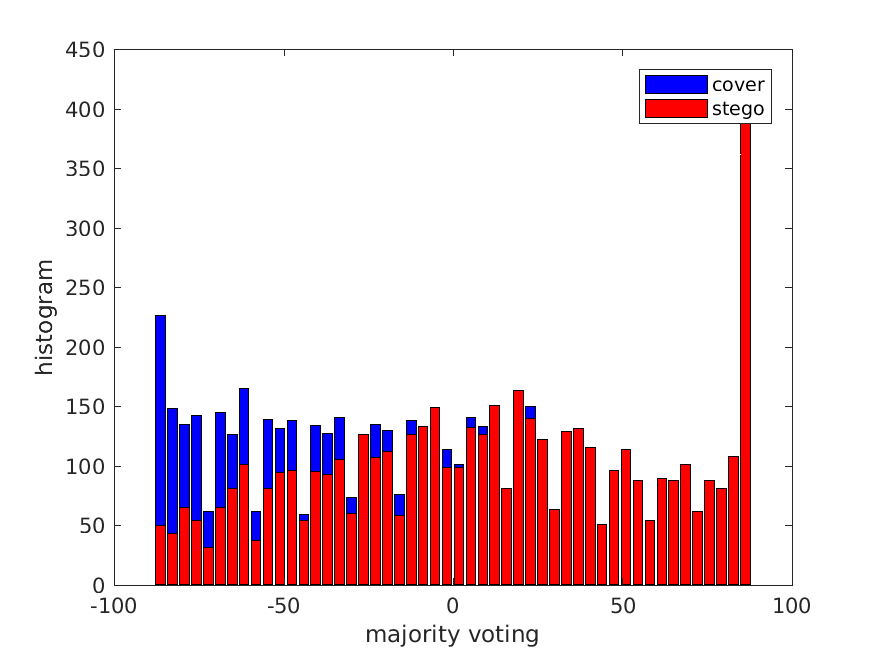
\includegraphics[width=.95\textwidth]{dados/figuras/voting.png}
%	\caption{Histograma da votação para o conjunto de treino M1 e de teste M.-.1.}
%    \label{fig:voting}
%\end{figure}


 
	
%\clearpage
\section{Esteganálise Baseada em CNN}

A abordagem de esteganálise com aprendizagem profunda empregada neste trabalho se baseia na proposta por \citeonline{cnn_base}, que utiliza uma rede neural convolucional (CNN) para predizer se uma imagem possui ou não uma mensagem escondida. A arquitetura da CNN utilizada pode ser vista na Figura \ref{fig:cnn_model}.

Inicialmente, é realizado um pré-processamento nas imagens, com a aplicação de um filtro passa-alta (HPF) com o seguinte \textit{kernel}:
	$$ \frac{1}{12}\left[
    \begin{array}{ccccc}
    -1 & 2 & -2 & 2 & -1 \\
    2 & -6 & 8 & -6 & 2 \\
    -2 & 8 & -12 & 8 & -2 \\
    2 & -6 & 8 & -6 & 2 \\
    -1 & 2 & -2 & 2 & -1
    \end{array}
    \right], $$ 
o qual serve para destacar o ruído residual, ajudando na esteganálise visto que os dados embutidos na imagem tendem a gerar distorções. Tal \textit{kernel} foi inicialmente empregado por \citeonline{kodovsky2011dangers} para esteganálise do algoritmo HUGO. Porém, por ter apresentado bons resultados também com outros algoritmos de esteganografia, é amplamente utilizado em vários modelos de esteganálise.

\begin{figure}[!htb]
	\centering
    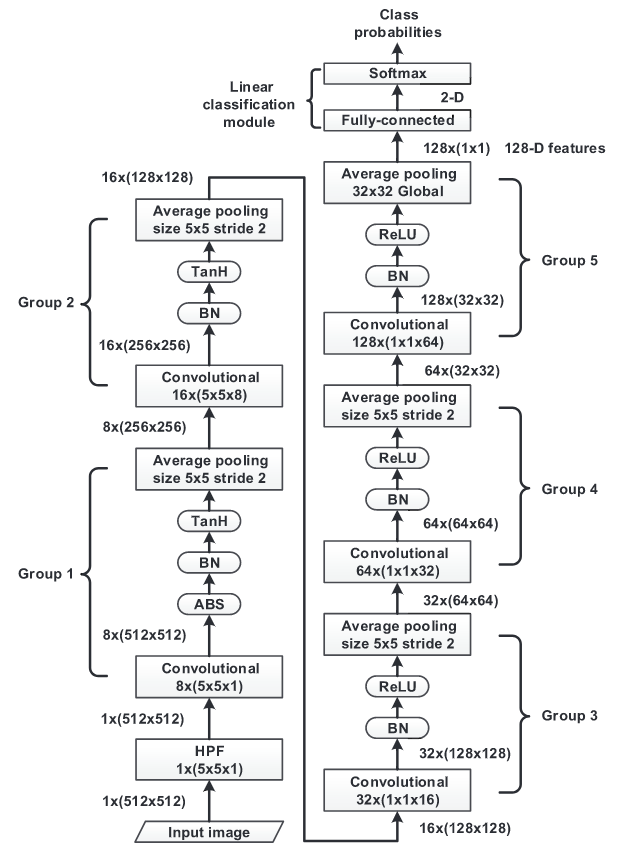
\includegraphics[width=.8\textwidth]{dados/figuras/cnn_model.png}
    \caption{Arquitetura da CNN utilizada. Dentro das caixas é mostrado o tipo da camada e seus parâmetros \cite{cnn_base}.}
    \label{fig:cnn_model}
\end{figure}
 
Após esse pré-processamento as imagens passam pela CNN, que pode ser dividida em seis grupos, sendo os cinco primeiros grupos convolucionais, e o último grupo de classificação linear. Os grupos convolucionais iniciam com uma camada de convolução e terminam com uma camada de média de subamostragem (\textit{average pooling}) com um \textit{kernel} de $5\times 5$ - com exceção do quinto grupo, onde a subamostragem é global.
 
Nos grupos 1 e 2, é utilizada a função de ativação não-linear tangente hiperbólica (TanH), enquanto nos grupos 3, 4 e 5 é usada a Unidade Retificada Linear (ReLU). No grupo 1 também é inserida uma camada de ativação modular (ABS), a qual calcula o valor absoluto de cada valor do mapa de características. Após essa camada, e após as camadas convolucionais nos outros grupos, é realizada uma normalização do conjunto (\textit{Batch Normalization} - BN) \cite{batch_normalization}, que objetiva impedir que o treinamento caia em um mínimo local.
 
Por fim, a parte de classificação linear recebe um mapa de 128 características em sua camada totalmente conectada, o que gera dois valores. Após a aplicação da função \textit{softmax} \cite{bishop2006pattern}, eles representam a probabilidade da imagem ser de cobertura ou estego.


\subsection{Experimentos}

Para o treinamento da rede, foram utilizados os 12 conjuntos listados na Tabela~\ref{tab:cenariosTrain}, gerados a partir da aplicação dos algoritmos HUGO, S-UNIWARD e MiPOD em 5000 imagens da base BOSSBase para diferentes \textit{payloads}.

As 5000 imagens de cada conjunto de treinamento foram divididas igualmente em cinco subconjuntos sem sobreposição, a partir dos quais foram gerados cinco modelos de CNN. Em cada um deles, um dos subconjuntos foi utilizado para validação e os quatro restantes para treinamento. Isto é feito como forma controlada de \textit{bootstrap aggregation} \cite{Breiman1996}, visando  criar uma combinação de classificadores. 

Na fase de testes, as imagens dos 28 cenários da Tabela~\ref{tab:cenariosTest} são classificadas pelas cinco CNNs treinadas. A predição final é calculada com base na média das probabilidades para cada imagem. Observe que esse procedimento é realizado para cada um dos 12 conjuntos de treinamento.

Cada uma das CNNs foi treinada por 30000 iterações, com lotes de 64 imagens (32 pares) para cada iteração. A taxa de aprendizagem (\textit{learning rate}) é inicializada em 0.001 sendo reduzida em 10\% a cada 5000 iterações. O \textit{momentum} é fixado em 0.9. O \textit{bias} foi desativado em todas as camadas convolucionais.

A implementação da CNN foi realizada em Python utilizando a biblioteca TensorFlow. Os experimentos foram executados em uma GeForce GTX Titan Xp, o tempo total de treinamento com cada conjunto foi de aproximadamente 22 horas e o tempo de uma bateria completa de testes, com os 28 cenários, foi de cerca de 2 horas.


\section{Comparação dos Resultados}
\label{sec:metricas}
	
Para comparar o desempenho da abordagem proposta neste trabalho em relação ao uso de um\textit{ Ensemble of Classifiers} (com descritor SRM), serão utilizadas duas métricas bastante disseminadas no âmbito da esteganálise: a acurácia e a área sob a curva \textit{Receiving Operating Characteristic} (ROC).

\subsection{Acurácia}

A acurácia de um classificador é uma medida simples dada pela quantidade de amostras classificadas de maneira correta divida pelo total de amostras. Essa medida é muito utilizada devido a sua simplicidade e objetividade.


\subsection{\textit{Area Under Curve} (AUC)}

Uma curva ROC é uma representação gráfica do desempenho de um classificador binário. Ela consiste em um gráfico da taxa de verdadeiros positivos versus a taxa de falsos positivos. %, variando um ou mais \textit{thresholds}. 
Ela é uma medida particularmente útil em domínios onde ocorre uma grande
desproporção entre as classes ou quando se deve considerar diferentes custos/benefícios para os diferentes erros/acertos de classificação. 

%Na Figura~\ref{fig:roc-example} podemos ver exemplos de curvas ROC.

%\begin{figure}[!ht]%
	%\center
	%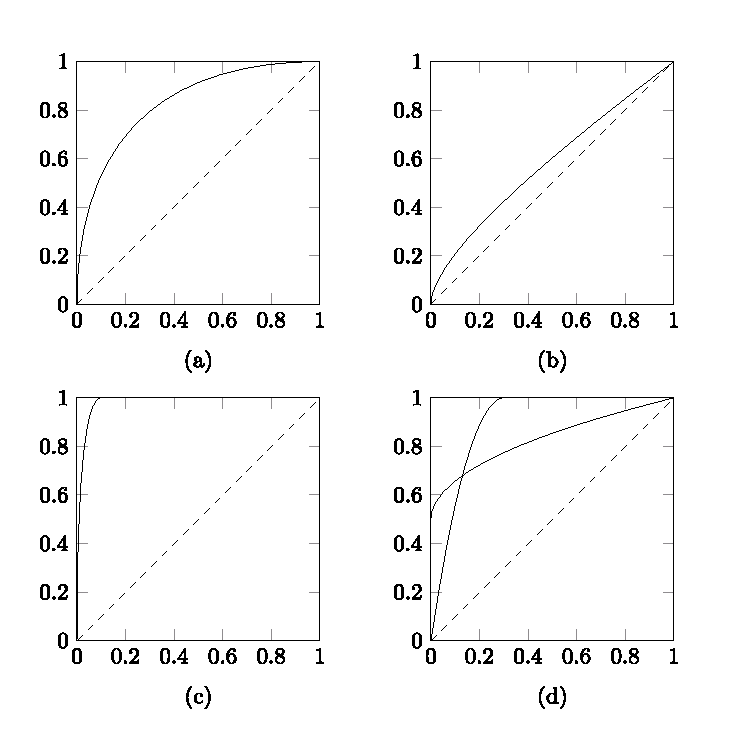
\includegraphics[width=0.8\textwidth]{dados/figuras/roc-examples.pdf}
	%\caption{Exemplos de curva ROC. Os eixos $x$ e $y$ representam nos quatro gráficos a probabilidade de falso positivo e a probabilidade de verdadeiro positivo, respectivamente. (a) Exemplo de curva ROC; (b) Example de um detector ruim; (c) Exemplo de um detector muito bom; (d) Curvas ROC de difícil comparação~\cite{fridrich2009steganography}.}
	%\label{fig:roc-example}
%\end{figure}

Dado que detectores diferentes podem ter intersecções entre suas curvas ROCs, causando dificuldades na comparação, pode-se considerar a área sob a curva (AUC - do inglês, \textit{Area Under Curve}) como medida de comparação.

Uma vez que a área abaixo da curva ROC é uma fração da área de um quadrado de
lado um, o seu valor, $p$, está sempre entre 0 e 1. Quando $p\approx 0,5$ a curva ROC está próxima à linha diagonal, ou seja, equivale ao classificador aleatório, e quando $p \approx 1$ a curva ROC está mais próxima dos detectores perfeitos.

%\begin{figure}[!htb]%
%	\center%
%	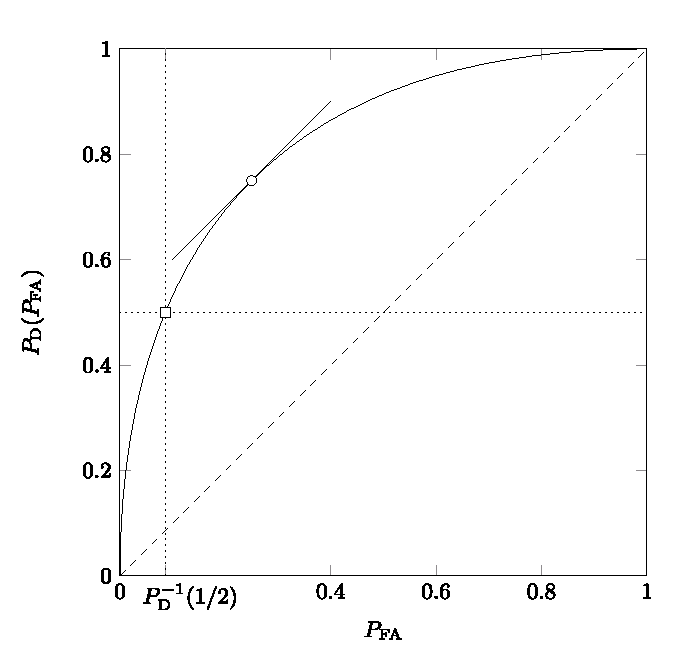
\includegraphics[width=0.75\textwidth]{dados/figuras/roc-pe-pd.pdf}
%	\caption{Medidas escalares para comparar detectores~\cite{fridrich2009steganography}. O quadrado corresponde ao critério $P_D^{-1}(1/2)$. O círculo corresponde ao critério $P_E$.}
%	\label{fig:roc-pe-pd}
%\end{figure}
